\documentclass{beamer}
\usetheme{Montpellier}
\usecolortheme{beaver}
\setbeamerfont{footnote}{size=\tiny}
\setbeamerfont{footnote mark}{size=\tiny}
\setbeamerfont{cite}{size=\tiny}
%Don't use default captions, footnote errors!
%https://tex.stackexchange.com/questions/43778/aberrant-footnote-numbering-behavior-with-footnoted-captions
%\setbeamerfont{caption}{size=\scriptsize}
%\setbeamertemplate{caption}{\insertcaption}
%\setbeamercolor{caption}{fg=blue}
%\setlength\abovecaptionskip{-5pt}


%To comment out sections
\usepackage{comment}

%bibliography
\usepackage[square,sort]{natbib}

%math
\usepackage{amsmath}

%symbols
\usepackage{gensymb}
\usepackage{upgreek}


%algorithm
\usepackage[algoruled]{algorithm2e}
%blue comments in algo.
\newcommand\mycommfont[1]{\footnotesize\ttfamily\textcolor{blue}{#1}}
\SetCommentSty{mycommfont}

%caption package for better behavior
\usepackage[skip=2pt]{caption}
\captionsetup{font={color=blue,scriptsize}}
\captionsetup{labelformat=empty,labelsep=none}
\captionsetup{justification=centering}

%For urls
\usepackage{hyperref}

%For tables
\usepackage{booktabs}
\usepackage{diagbox}



% Define some common variables
\def\micron{$\upmu$m}
\def\deltaz{\delta_{z}} % depth resolution
\def\drn{dr_{N}} % outermost zone width
\def\rn{r_{N}} % zone plate radius
\def\NA{\mbox{N.A.}}
\def\deltaz{\delta_{z}} % depth resolution
\def\deltares{\delta_{r}} % Spatial resolution
\def\tzp{t_{\rm zp}} % Zone plate thickness
\def\tzpopt{t_{\rm zp,opt}} % Optimum thickness
\def\thetazp{\theta} % Zone plate tilt
\def\thetabragg{\theta_{\rm B}} % Bragg angle

\def\thetaellapproxu{\theta_{u}} % Rayleigh quarter wave tilt limit
\def\thetaellapproxl{\theta_{l}} % Rayleigh quarter wave tilt limit

\def\thetaellc{\theta_c} % tilt limit if coma dominates
\def\thetaella{\theta_a} % tilt limit of astigmatism dominates

\def\thetadof{\theta_{\rm DOF}} % tilt limit via depth of focus

\def\ellexactu{\ell_{u}^{\prime}}
\def\ellexactl{\ell_{l}^{\prime}}

\def\ellapproxu{\ell_{u}}
\def\ellapproxl{\ell_{l}}
\def\ellapprox0{\ell_{0}}

\def\ellapproxc{\ell_{c}}
\def\ellapproxa{\ell_{a}}

\def\ellmyers{\ell_{\rm m}}
\def\ellmyersprime{\ell_{\rm m}^{\prime}}

\def\dof{\mbox{DOF}}
\def\thetafield{\theta_{f}}
\def\npix{N_{x}}
\def\pixelsize{\Delta_{x}}
\def\pixelsizeout{\Delta_{x}^{\prime}}
\def\pixeldepth{\Delta_{z}}
\def\pixelphase{\varphi_{x}}
\def\nzpix{N_{z}}
\def\voxelfraction{\chi}
\def\pixeldepthkc{\Delta_{z,Q}}
\def\qkleincook{Q} % Klein--Cook parameter
\def\realpix{\Delta_{r}} % real space pixel size in CDI
% Define some common variables
\def\micron{$\upmu$m}
\def\deltaz{\delta_{z}} % depth resolution
\def\drn{dr_{N}} % outermost zone width
\def\rn{r_{N}} % zone plate radius
\def\NA{\mbox{N.A.}}
\def\deltaz{\delta_{z}} % depth resolution
\def\deltares{\delta_{r}} % Spatial resolution
\def\tzp{t_{\rm zp}} % Zone plate thickness
\def\tzpopt{t_{\rm zp,opt}} % Optimum thickness
\def\thetazp{\theta} % Zone plate tilt
\def\thetabragg{\theta_{\rm B}} % Bragg angle

\def\thetaellapproxu{\theta_{u}} % Rayleigh quarter wave tilt limit
\def\thetaellapproxl{\theta_{l}} % Rayleigh quarter wave tilt limit

\def\thetaellc{\theta_c} % tilt limit if coma dominates
\def\thetaella{\theta_a} % tilt limit of astigmatism dominates

\def\thetadof{\theta_{\rm DOF}} % tilt limit via depth of focus

\def\ellexactu{\ell_{u}^{\prime}}
\def\ellexactl{\ell_{l}^{\prime}}

\def\ellapproxu{\ell_{u}}
\def\ellapproxl{\ell_{l}}
\def\ellapprox0{\ell_{0}}

\def\ellapproxc{\ell_{c}}
\def\ellapproxa{\ell_{a}}

\def\ellmyers{\ell_{\rm m}}
\def\ellmyersprime{\ell_{\rm m}^{\prime}}

\def\dof{\mbox{DOF}}
\def\thetafield{\theta_{f}}
\def\npix{N_{x}}
\def\pixelsize{\Delta_{x}}
\def\pixelsizeout{\Delta_{x}^{\prime}}
\def\pixeldepth{\Delta_{z}}
\def\pixelphase{\varphi_{x}}
\def\nzpix{N_{z}}
\def\voxelfraction{\chi}
\def\pixeldepthkc{\Delta_{z,Q}}
\def\qkleincook{Q} % Klein--Cook parameter
\def\realpix{\Delta_{r}} % real space pixel size in CDI



\title{Effect of tilt on zone plate performance}
\author{Sajid Ali\inst{1} \& Chris Jacobsen\inst{2}}	
\institute[NU] 
{\inst{1}%
  Applied Physics\\
  Northwestern University\\
\inst{2}%	
	X-ray Science Divison\\
	Argonne National Lab}
\date{\today}
% If you have a file called "university-logo-filename.xxx", where xxx
% is a graphic format that can be processed by latex or pdflatex,
% resp., then you can add a logo as follows:

% \pgfdeclareimage[height=0.5cm]{university-logo}{university-logo-filename}
% \logo{\pgfuseimage{university-logo}}

% Delete this, if you do not want the table of contents to pop up at
% the beginning of each subsection:
\AtBeginSubsection[]
{
  \begin{frame}<beamer>{Outline}
    \tableofcontents[currentsection,currentsubsection]
  \end{frame}
}
\AtBeginSection[]{
	\begin{frame}
		\vfill
		\centering
		\begin{beamercolorbox}[sep=8pt,center,shadow=true,rounded=true]{title}
			\usebeamerfont{title}\insertsectionhead\par%
		\end{beamercolorbox}
		\vfill
	\end{frame}
}

% Let's get started
\begin{document}

\begin{frame}
  \titlepage
\end{frame}

\begin{frame}{Outline}
  \tableofcontents[hideallsubsections]
  % You might wish to add the option [pausesections]
\end{frame}

% Section and subsections will appear in the presentation overview
% and table of contents.

\section{Introduction}
\subsection{Background}
\begin{frame}{Focusing X-Rays}
	\begin{block}{}
		\begin{columns}[onlytextwidth,T]
			\column{\dimexpr\linewidth-30mm-10mm}
			\begin{itemize}
			\item Ref. index$\rightarrow$ complex,slightly $<$ 1
			\item Zone plates$\rightarrow$ monochromatic diffractive optics.
			\item Alternate rings of low/high ref. index materials placed such that  outgoing waves interfere constructively.			
			\end{itemize}
			\column{30mm}
			\begin{figure}
				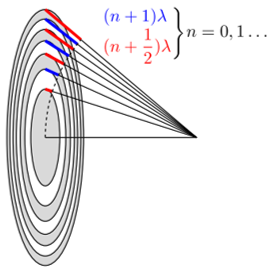
\includegraphics[width=40mm]{zp}
				\caption{Illustration of zone plate \footnotemark}
			\end{figure}
		\end{columns}
	\footnotetext{\cite{jacobsen_2019}}
	\end{block}
\end{frame}


\begin{frame}{Factors affecting efficiency \& resolution}
	\begin{block}{}
		\begin{columns}[onlytextwidth,T]
			\column{\dimexpr\linewidth-30mm-10mm}
			\begin{itemize}
				\item Spatial resolution limited to finest, outermost zone width.\footnotemark
				\item Zones must be thick enough along beam direction to produce a phase shift of $\pi$, several um at hard x-ray energy.\footnotemark
				%\item $\tzpopt \simeq \frac{\lambda}{2\delta}\left(1-\frac{2\beta}{\pi
				%	\delta}\right)$
			\end{itemize}
			\column{30mm}
			\begin{figure}
				\hspace*{-1.1cm}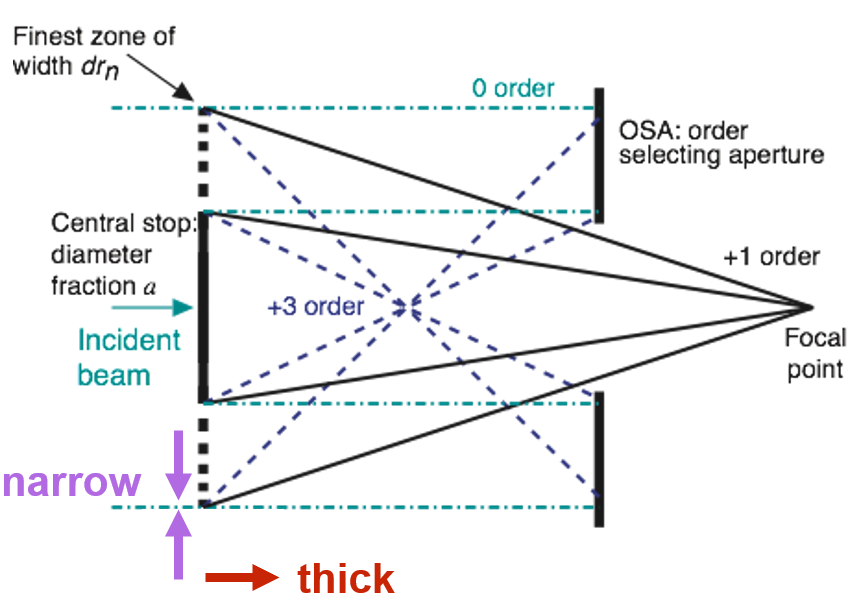
\includegraphics[width=50mm]{zp_chris}
				\caption{Efficiency \& resolution for first order focus\footnotemark}
			\end{figure}
		\end{columns}
		\end{block}
		\addtocounter{footnote}{-2}
			\footnotetext{\cite{myers_ajp_1951,baez_josa_1952}}
		\stepcounter{footnote}\stepcounter{footnote}
		
		\addtocounter{footnote}{-1}
			\footnotetext{\cite{kirz_josa_1974}}
		\stepcounter{footnote}
		
		\footnotetext{\cite{jacobsen_2019}}
\end{frame}

\begin{frame}{Scalar theory is not enough}
	\begin{block}{}
		\begin{columns}[onlytextwidth,T]
			\column{\dimexpr\linewidth-30mm-10mm}
			\begin{itemize}
				\item Scalar approximation assumption $\rightarrow$ interaction between x-rays and the optic can be treated as one-step diffraction. 
				\item Klein-Cook param. : $Q_{K-C}$ indicator of 
				"diffraction regime"\footnotemark.
			\end{itemize}
			\column{30mm}
			\begin{figure}
				\vspace*{-0.75cm}\hspace*{-0.75cm}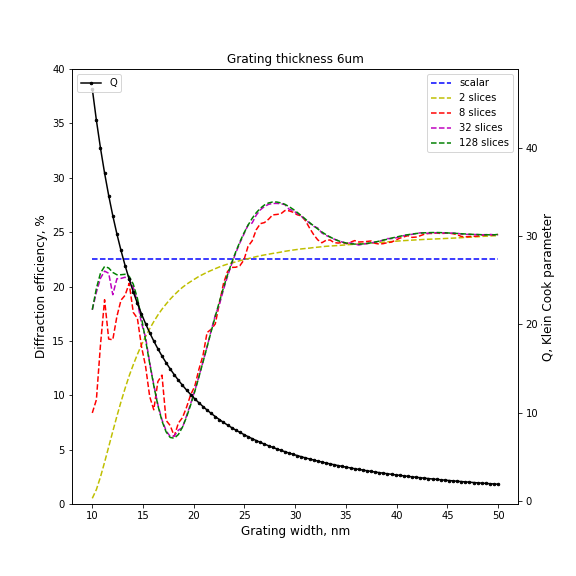
\includegraphics[width=45mm]{grating}
				\caption{Volume effects in 1d gratings}
			\end{figure}
		\end{columns}
	\footnotetext{\cite{klein_ieeetsu_1967}}
	%\footnotetext{\cite{Li17}}
	\end{block}
\end{frame}

\subsection{Motivation}
\begin{frame}{Need for tilt misalignment study \footnotemark 	\footnotetext{Tilting zones to local bragg angle is not considered here. }}
	\begin{itemize}
		\item As aspect ratios of zone plates go up\footnotemark \footnotetext{\cite{chang_natcomm_2014,parfeniukas_spie_2017,li_jvstb_2017}} , degredation of performance due to tilt misalignment becomes more prominent.
		\item Analytic limits\footnotemark 	\footnotetext{\cite{myers_ajp_1951,young_josa_1972}} from literature do not account for volume diffraction effects.
	\end{itemize}

\end{frame}


\section{Analytic limits}
\begin{frame}{Analytic limits}
	\begin{block}{}
		\begin{columns}[onlytextwidth,T]
			\column{\dimexpr\linewidth-30mm-10mm}
			\begin{itemize}
				\item Based on path length deviation (from no tilt) between marginal, axial ray\footnotemark $\rightarrow$ $\ellexactu,\ellexactl$.
				\item Simplified expressions for path length deviation 
			   \begin{itemize}
					\item $\ellapproxu = (\ellapprox0) + \ellapproxc \theta-\ellapproxa
					\theta^{2}$
					\item $\ellapproxl = (\ellapprox0) + \ellapproxc \theta+\ellapproxa
					\theta^{2}$
				\end{itemize}
			\item $\ellapprox0$ $\rightarrow$ convergence to focus, $\ellapproxc$ $\rightarrow$ coma, $\ellapproxa$ $\rightarrow$
			astigmatism \& field curvature\footnotemark.
			\end{itemize}
			\column{30mm}
			\begin{figure}
				\hspace*{-1cm}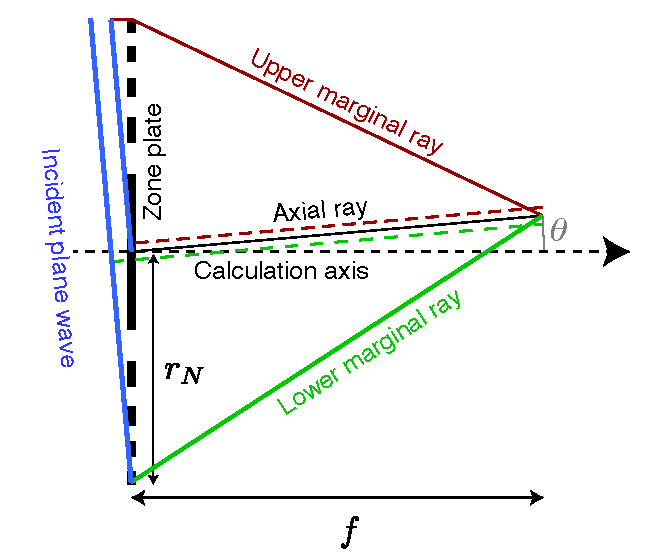
\includegraphics[width=50mm]{zp_schematic}
				\caption{Path length schematic.}
			\end{figure}
		\end{columns}
	\addtocounter{footnote}{-1}
		\footnotetext{\cite{myers_ajp_1951,young_josa_1972}}
	\stepcounter{footnote}
	\footnotetext{referred to hereafter as astigmatism only.}
	\end{block}
\end{frame}


\begin{frame}{Expected behavior}
	\begin{itemize}
		\item $\frac{\ellapproxa \theta^{2}}{\ellapproxc\theta} \propto\frac{\theta}{\scriptsize{N.A.}}$, $\scriptsize{N.A.}$ $\rightarrow$ numerical aperture.
		\item RQW limit\footnotemark : $\thetaellc < \frac{1}{2N\,\scriptsize{N.A.}}$ $|$ $\thetaella < \frac{1}{\sqrt{3N}}$, $N$ $\rightarrow$ number of zones.
		\begin{center}
			\begin{figure}
				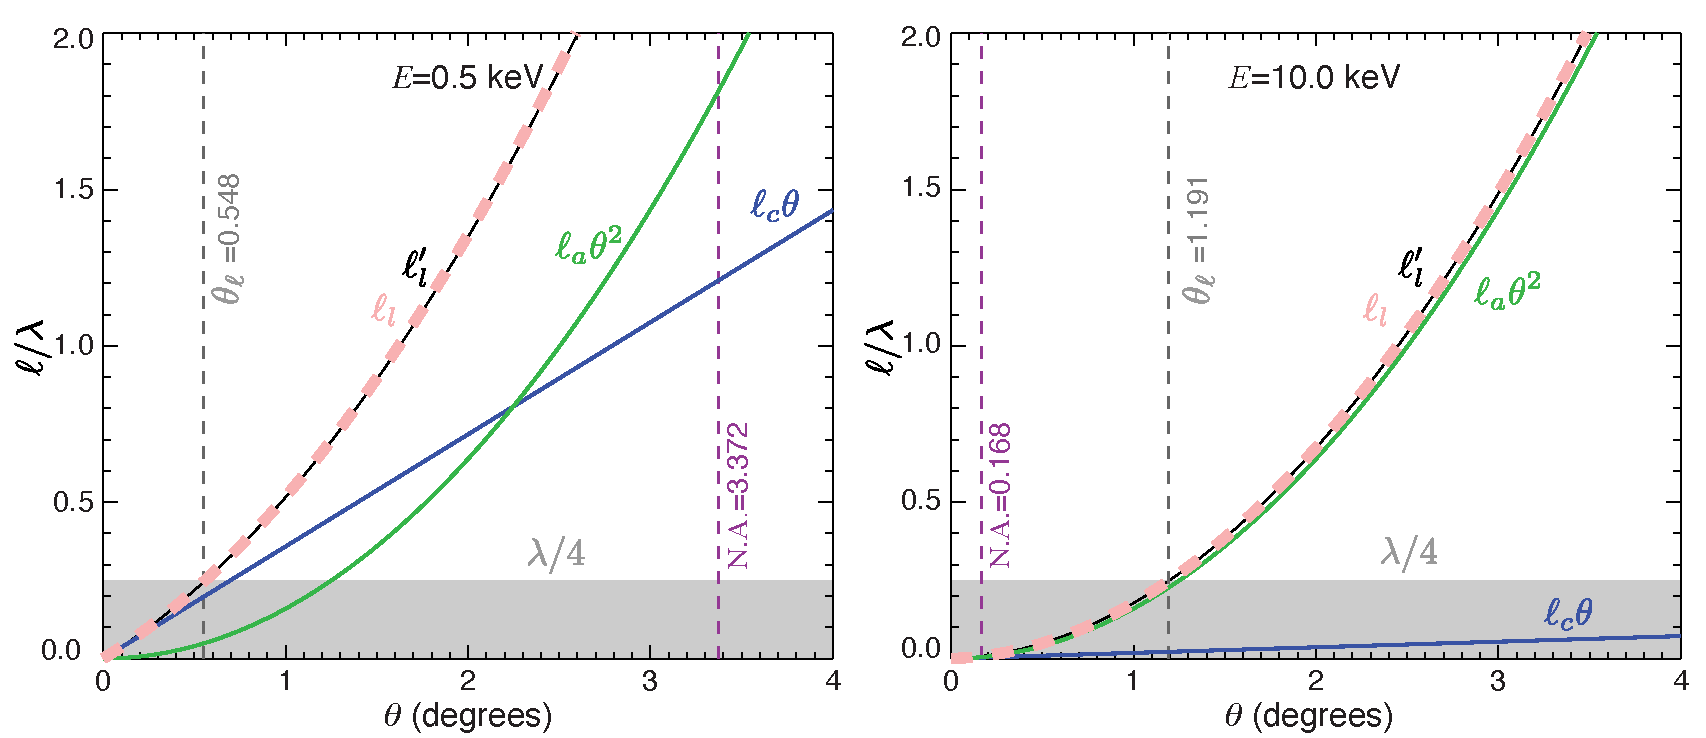
\includegraphics[scale=0.35]{path_length_terms}
				\caption{Path length terms}	
			\end{figure}
		\end{center}
	\end{itemize}
	\footnotetext{Rayleigh Quarter Wave Criterion}
\end{frame}


\section{Implementation}
\subsection{Creating zone plates}
\begin{frame}{Partial Filling}
	\begin{itemize}
		\item Binary fill on a smaller pixel grid, then downsample!
		\begin{center}
			\begin{figure}
				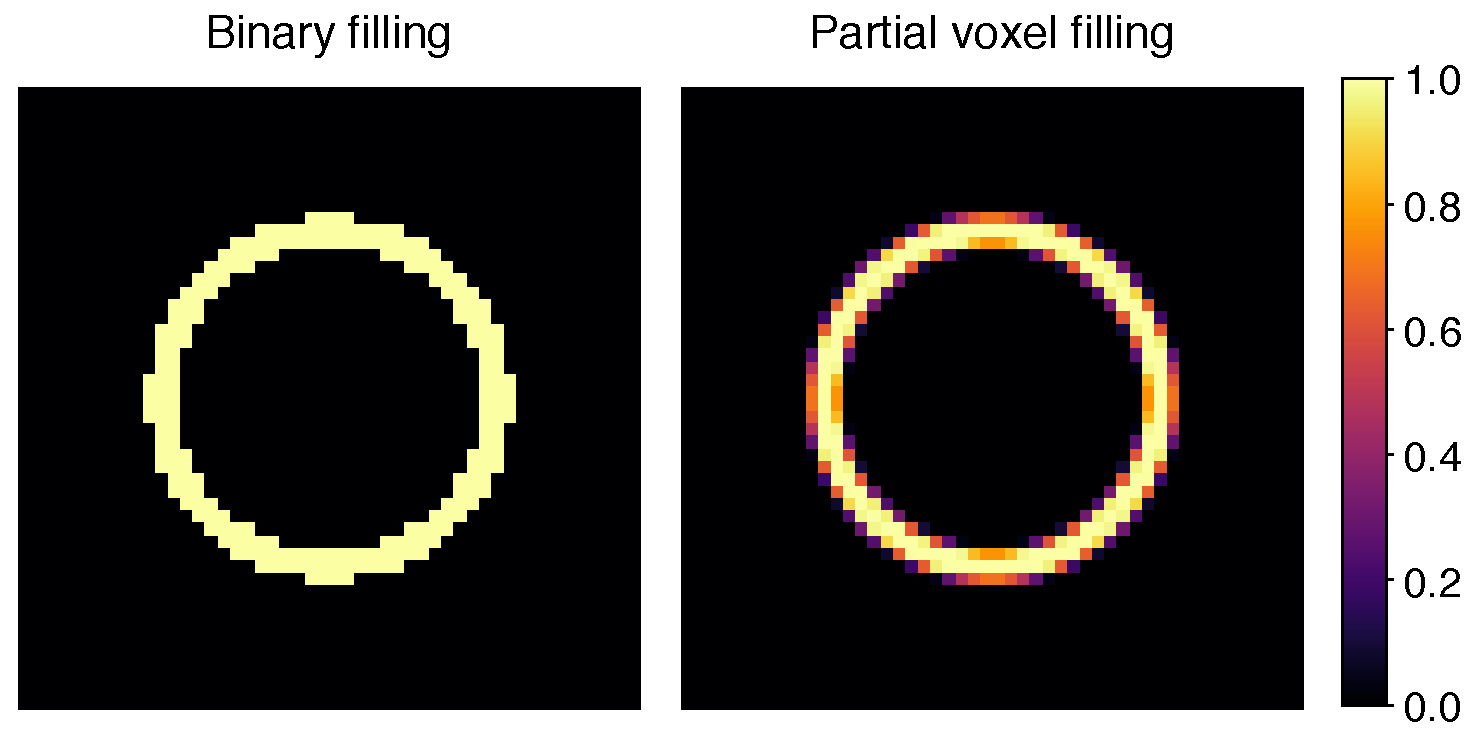
\includegraphics[scale=0.35]{partial_fill}
				\caption{Partial fill}	
			\end{figure}
		\end{center}
	\end{itemize}
\end{frame}


\subsection{Multislice}
\begin{frame}{Multislice}
		\begin{itemize}
			\item "Slice" the object into multiple thin sections\footnotemark.
			\item Agrees with rigorous coupled wave theory\footnotemark.
		\end{itemize}
		\begin{figure}
			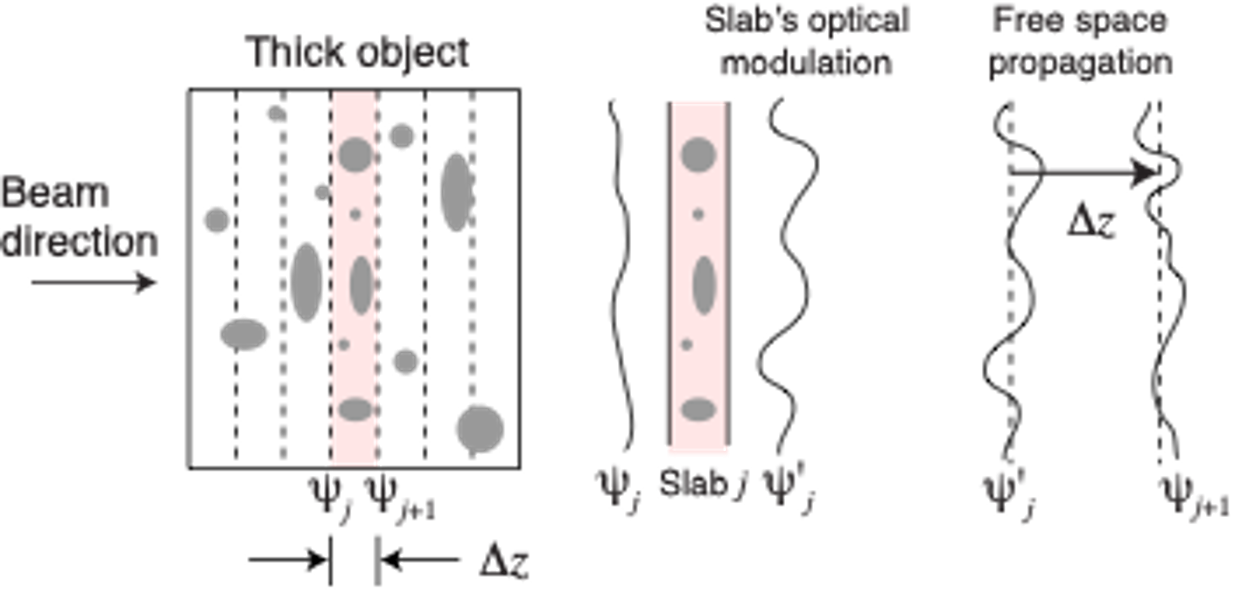
\includegraphics[scale=0.25]{ms}
			\caption{Multi-slice schematic \footnotemark }
		\end{figure}
	
		\addtocounter{footnote}{-2}
			\footnotetext{\cite{cowley_actacryst_1957}, \cite{ishizuka_aca_1977}, also known as beam prop. meth. \cite{vanroey_josa_1981}}
		\stepcounter{footnote}\stepcounter{footnote}
		\addtocounter{footnote}{-1}
			\footnotetext{\cite{li_optexp_2017}}
		\stepcounter{footnote}
		\footnotetext{\cite{jacobsen_2019}}
\end{frame}

\begin{frame}
	\begin{block}{}
		\begin{columns}[totalwidth=1.1\textwidth,c]
			\column{.6\textwidth}
			\scalebox{0.6}{
				\begin{algorithm}[H] 
					% This is to hide end and get the last vertical line straight
					\SetAlgoLined\DontPrintSemicolon
					
					\SetKwFunction{SliceDiff}{SliceDiff}
					\SetKwFunction{PropShort}{PropShort}
					\SetKwFunction{PropLong}{PropLong}
					
					\tcc{initialize}
					$\psi(x,y) \xleftarrow{} 1$\;
					\tcc{diffraction within optic}
					\For{n=1,N}{ 	
						\SliceDiff{n}\;
						\PropShort{$\pixeldepth$}\;
					}
					\tcc{Propagate exit wave by a focal length $f$ to the focal plane}
					\PropLong{$f$} \;
					\caption{Optic simulation using the multislice method.}
				\end{algorithm}
			}
			
			\column{0.9\textwidth}
			\scalebox{0.6}{
				\begin{algorithm}[H]
					%This is to hide Begin keyword
					\SetKwProg{myproc}{Procedure}{}{}
					\myproc{\SliceDiff{n}}{
						\tcc{Apply refractive effect of slice using }	
						$\psi(x,y) = \psi(x,y) \odot \exp\Bigl[i\, \frac{2\pi \pixeldepth}{\lambda} \bigl(\delta(x,y)+i\beta(x,y)\bigr)\Bigr]$ \;
						\KwRet\;}
					
					\SetKwProg{myproc}{Procedure}{}{}
					\myproc{\PropShort{$\pixeldepth$}}{
						\tcc{Free space propagation from source $s$ to destination $d$ plane}	
						$\psi_{s}(x,y) \xrightarrow{\mathcal{F}}\Psi(u,v)$\;
						$\Psi(u,v) = \Psi(u,v) \odot \exp\Bigl[-i\, \frac{2\pi \pixeldepth}{\lambda} \sqrt{1-\lambda^{2}(u^{2}+v^{2})}\Bigr]$\;
						$\Psi(u,v) \xrightarrow{\mathcal{F}^{-1}}\psi_d(x,y)$\;
						\KwRet\;}
					
					\SetKwProg{myproc}{Procedure}{}{}
					\myproc{\PropLong{$f$}}{
						\tcc{Free space propagation from source $s$ to destination $d$ plane}	
						$\psi^{\prime}(x,y) = \psi_{s}(x,y) \odot \exp\Bigl[-i\,\frac{2\pi f}{\lambda}  \sqrt{x_{s}^{2}+x_{s}^{2}+f^{2}}\Bigr]$\;
						$\psi^{\prime}(x,y) \xrightarrow{\mathcal{F}} \Psi^{\prime}(x,y)$\;
						$\Psi_{d}(x,y) = \Psi^{\prime}(x,y) \odot \exp\Bigl[-i\,\frac{2\pi f}{\lambda} \sqrt{x_{d}^{2}+x_{d}^{2}+f^{2}}\Bigr]$\;
						$\psi_{d}(x,y) = \frac{i\pixelsize^2}{\lambda f} \Psi_{d}(x,y)$\;
						\KwRet\;}
					%				\caption{Optic simulation using the multislice method.}
				\end{algorithm}
			}
		\end{columns}
	\end{block}
\end{frame}


\subsection{Simulating tilt misalignment}
\begin{frame}{Approaches to simulating tilt misalignment}
	\begin{block}{}
		\begin{columns}[onlytextwidth,T]
			\column{\dimexpr\linewidth-30mm-10mm}
			\begin{itemize}
				\item Two methods to simulating tilt.
				\begin{itemize}
					\item Optic aligned.
					\item Wavefiled aligned.
				\end{itemize}
			\item Optic aligned $\rightarrow$ simple, but limited to cases where output grid can capture focus.	
			\item Wavefiled aligned $\rightarrow $ time consuming but no limit on tilt angle.
			\end{itemize}
			\column{30mm}
			\begin{figure}
				\vspace*{-1cm}\hspace*{-1.25cm}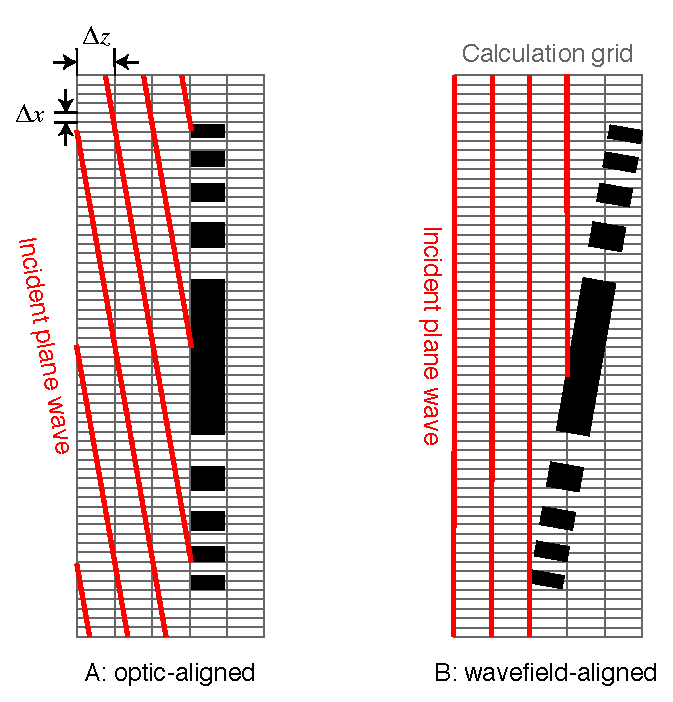
\includegraphics[width=50mm]{tilted_zp_grids}
				\caption{Tilt schematic}
			\end{figure}
		\end{columns}
	\end{block}
\end{frame}



\begin{frame}{Optic aligned approach}
	\begin{itemize}
		\item Apply a phase of $\frac{2\pi}{\lambda} x \tan(\theta)$ at each pixel.
	\end{itemize}
	\begin{center}
		\scalebox{0.65}{
			\begin{algorithm}[H] 				
				\SetAlgoLined\DontPrintSemicolon \SetKwFunction{AddPhase}{AddPhase}
				
				\SetKwFunction{SliceDiff}{SliceDiff}
				\SetKwFunction{PropShort}{PropShort}
				\SetKwFunction{PropLong}{PropLong}
				
				\tcc{For each angle in range of interest}	
				\For{i=1,K}{ 	
					
				\tcc{initialize} \AddPhase{$\theta$}\;
				\tcc{diffraction within optic}
				\For{n=1,N}{
					\SliceDiff{n}\;
					\PropShort{$\pixeldepth$}\;
				}
				\tcc{Propagate exit wave by a focal length $f$ to the focal plane}
				\PropLong{$f$} \;
				}
				\SetKwProg{myproc}{Procedure}{}{}
				\myproc{\AddPhase{$\theta$}}{
					\tcc{Apply phase to mimic tilt misalignment}	
					$\psi(x,y) \xleftarrow{} 1$ \;
					$\pixelphase = \frac{2\pi}{\lambda}\, \tan(\theta) x$ \;
					$\psi(x,y) = \psi(x,y) \odot \exp[i \pixelphase]$ \;
					\KwRet\;}
				
				\caption{Optic-aligned approach.}
			\end{algorithm}
		}
	\end{center}
\end{frame}


\begin{frame}{Wavefield aligned approach}
	\begin{itemize}
		\item Reduce the size of 2D grid to essential area.
		\item Duplicate slices along propagation direction to create isotropic grid.
		\item Rotate zone plate relative to grid.
		\item Collapse the grid back along the propagation direction.
	\end{itemize}
\end{frame}

\begin{frame}
	\begin{block}{}
		\begin{columns}[totalwidth=1.1\textwidth,c]
			\column{.6\textwidth}
			\scalebox{0.6}{
				\begin{algorithm}[H] 
					\SetAlgoLined\DontPrintSemicolon
					
					\SetKwFunction{Reduce}{Reduce}
					\SetKwFunction{Rotate}{Rotate}
					\SetKwFunction{Extract}{Extract}
					\SetKwFunction{SliceDiff}{SliceDiff}
					\SetKwFunction{PropTF}{PropTF}
					\SetKwFunction{PropFT}{PropFT}
					
					\tcc{Reduce the pattern down to essential area.}	
					\Reduce(pattern) \;
					
					\tcc{For each angle in range of interest}	
					\For{i=1,K}{ 	
						\Rotate(pattern\_reduced)\;
						\tcc{For each slice in a zone plate at a given tilt misalignment perform multislice simulation}	
						\For{n=1,N}{ 	
							\Extract(pattern\_reduced)\;
							\SliceDiff{n}\;
							\PropShort{$\Delta z$}\;	
						}
						\PropLong{f}\;
					}
					\caption{Wavefield-aligned approach.}
				\end{algorithm}
			}
			
			\column{0.9\textwidth}
			\scalebox{0.6}{
				\begin{algorithm}[H]
					\SetKwProg{myproc}{Procedure}{}{}
					\myproc{\Reduce(pattern)}{
						\tcc{Extract relevant part of zone plate}
						\tcc{choose and save appropriate parameters viz. number of slices, step size along propagation direction}
						pattern $\xrightarrow{}$pattern\_reduced \;
						\KwRet\;}
					\SetKwProg{myproc}{Procedure}{}{}
					
					\myproc{\Rotate(pattern\_reduced)}{
						\tcc{Rotate zone plate pattern}	
						\tcc{Expand the number of slices along direction of propagation to form an isotropic three dimensional grid.}
						pattern\_reduced $\xrightarrow{\text{Expand}}$ pattern\_isometric\;
						\tcc{Rrotate along axis of rotation}
						pattern\_isometric $\xrightarrow{\text{Rotation}}$ pattern\_isometric\;
						\tcc{reduce number of slices to number of slices for propagation.}
						pattern\_isometric $\xrightarrow{\text{Collapse}}$ pattern\_reduced\;
						\KwRet\;}
					
					\myproc{\Extract(pattern\_reduced)}{
						\tcc{Extract zone plate pattern at slice, expand back to grid size neede for propagation.}
						pattern\_reduced $\xrightarrow{}$pattern \;
						\KwRet\;}
				\end{algorithm}
			}
		\end{columns}
	\end{block}
\end{frame}

\subsection{Parameters}
\begin{frame}
	\begin{center}
	\scalebox{0.65}{
		\begin{tabular}{p{5.5cm} r r}
			\toprule
			\diagbox{Parameter}{Regime} & Soft X ray & Hard X ray \\
			\midrule
			
			Photon energy & 0.5 keV & 10 keV \\ 
			\midrule
			
			Outermost zone width $\drn$ & 21.09 nm & 21.07 nm \\ 
			\midrule
			
			Diameter $2\rn$ & 58.90 \micron{} & 58.88 \micron{} \\ 
			\midrule
			
			Pixels $\npix$ & 55,296 & 55,296 \\ 
			\midrule
			
			Input array pixel size $\pixelsize$ & 4.73 nm & 4.73 nm \\
			\midrule
			
			Output array pixel size $\pixelsizeout$ & 4.73 nm & 4.74 nm \\ \midrule
			
			Focal length $f$ & 0.5 mm & 10 mm \\ \midrule
			
			Numerical aperture $\NA$ & 3.372\degree{} & 0.168\degree{} \\ \midrule
			
						
			Bragg tilt angle\footnotemark  $\thetabragg(\rn)$
			& 1.687\degree{} & 0.084\degree{} \\ \midrule
			
			Aberration tilt limit $\thetaellapproxl$ &
			0.548\degree{} & 1.191\degree{} \\ \midrule
			
			
			Max tilt $\thetafield$ for optic-alig. approach& 10.90\degree{} & 0.75\degree{} \\ \midrule
			
			Optimum thickness $\tzpopt$
			& 0.098 \micron{}
			& 1.975 \micron{} \\ \midrule
			
			$\tzp$ for $\qkleincook=0.333$ & 0.038 \micron{} & 0.759 \micron{} \\
			\midrule
			
			$\tzp$ for $\qkleincook=3.333$ & 0.381 \micron{}  & 7.594 \micron{} \\
			\midrule
			
			$\tzp$ for $\qkleincook=10$ & 1.142 \micron{} & 22.782 \micron{} \\ 
			
			\bottomrule 
			
			\end{tabular}
		}
		\end{center}
	
	\footnotetext{For outermost zones}
\end{frame}



\section{Results}
\subsection{Soft x-ray}
\begin{frame}{Qualitative performance}
	\begin{itemize}
		\item Coma predicted.
	\end{itemize}
		\begin{center}
			\begin{figure}
				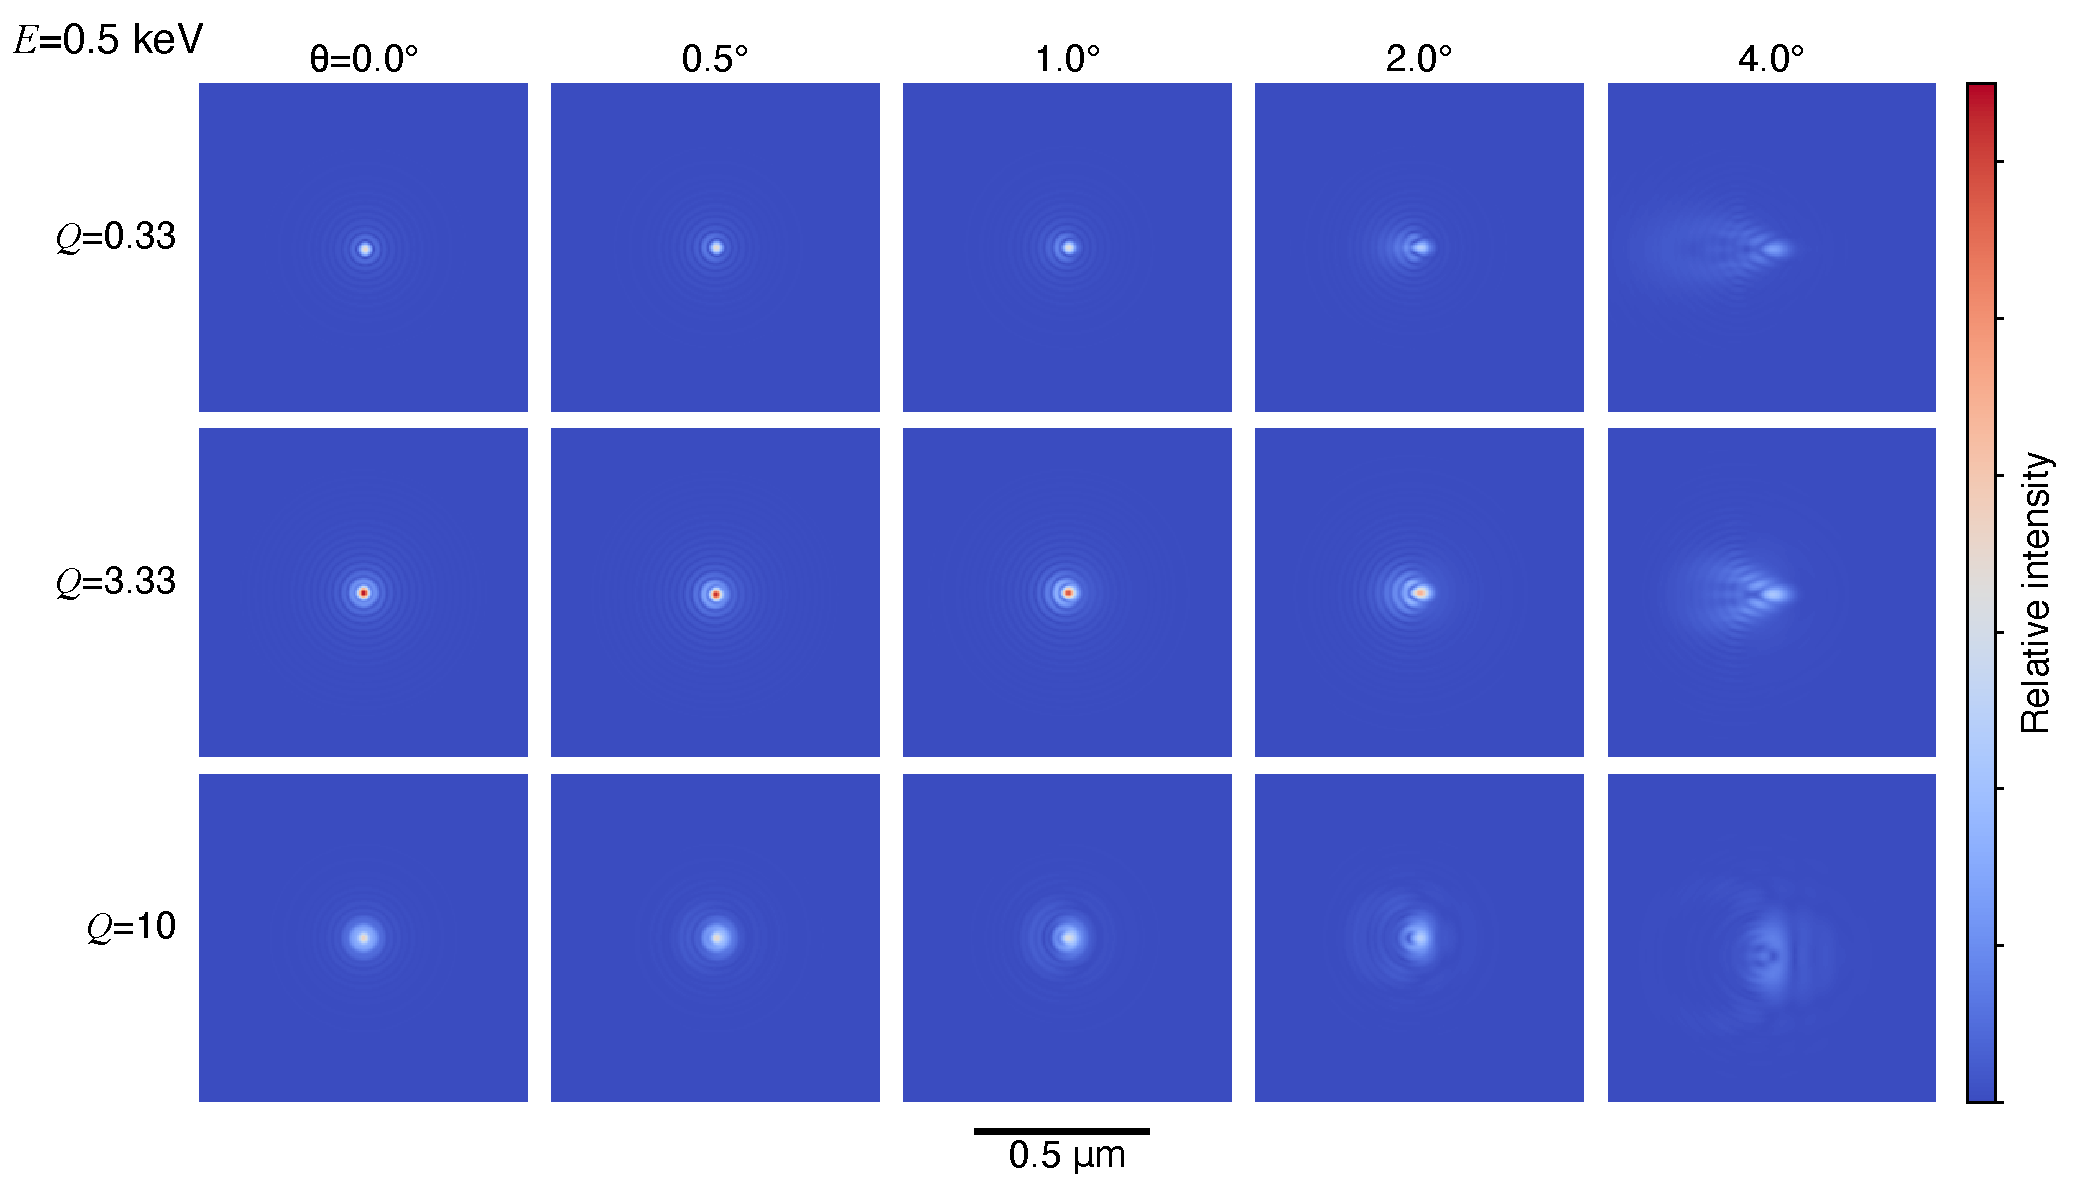
\includegraphics[scale=0.29]{foc_spot_half}
				\caption{Focal Profile}
			\end{figure}
		\end{center}
\end{frame}

\begin{frame}{Quantitative performance}
		\begin{center}
			\begin{figure}
				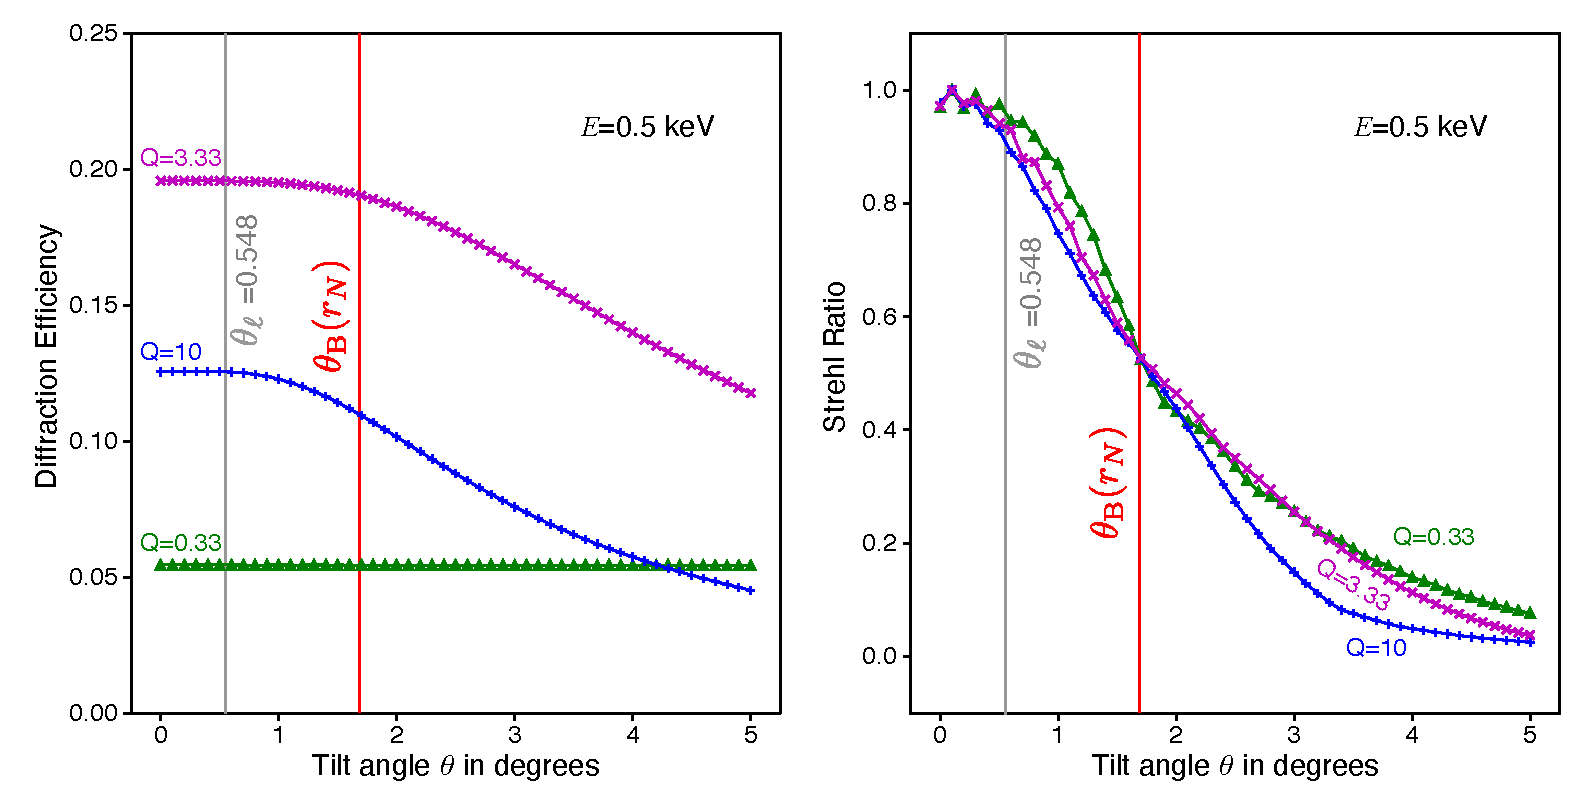
\includegraphics[scale=0.4]{tilt_plot_half}
			\end{figure}
		\end{center}
\end{frame}

\subsection{Hard x-ray}
\begin{frame}{Qualitative performance}
	\begin{itemize}
		\item Astigmatism predicted.
	\end{itemize}
		\begin{center}
			\begin{figure}
				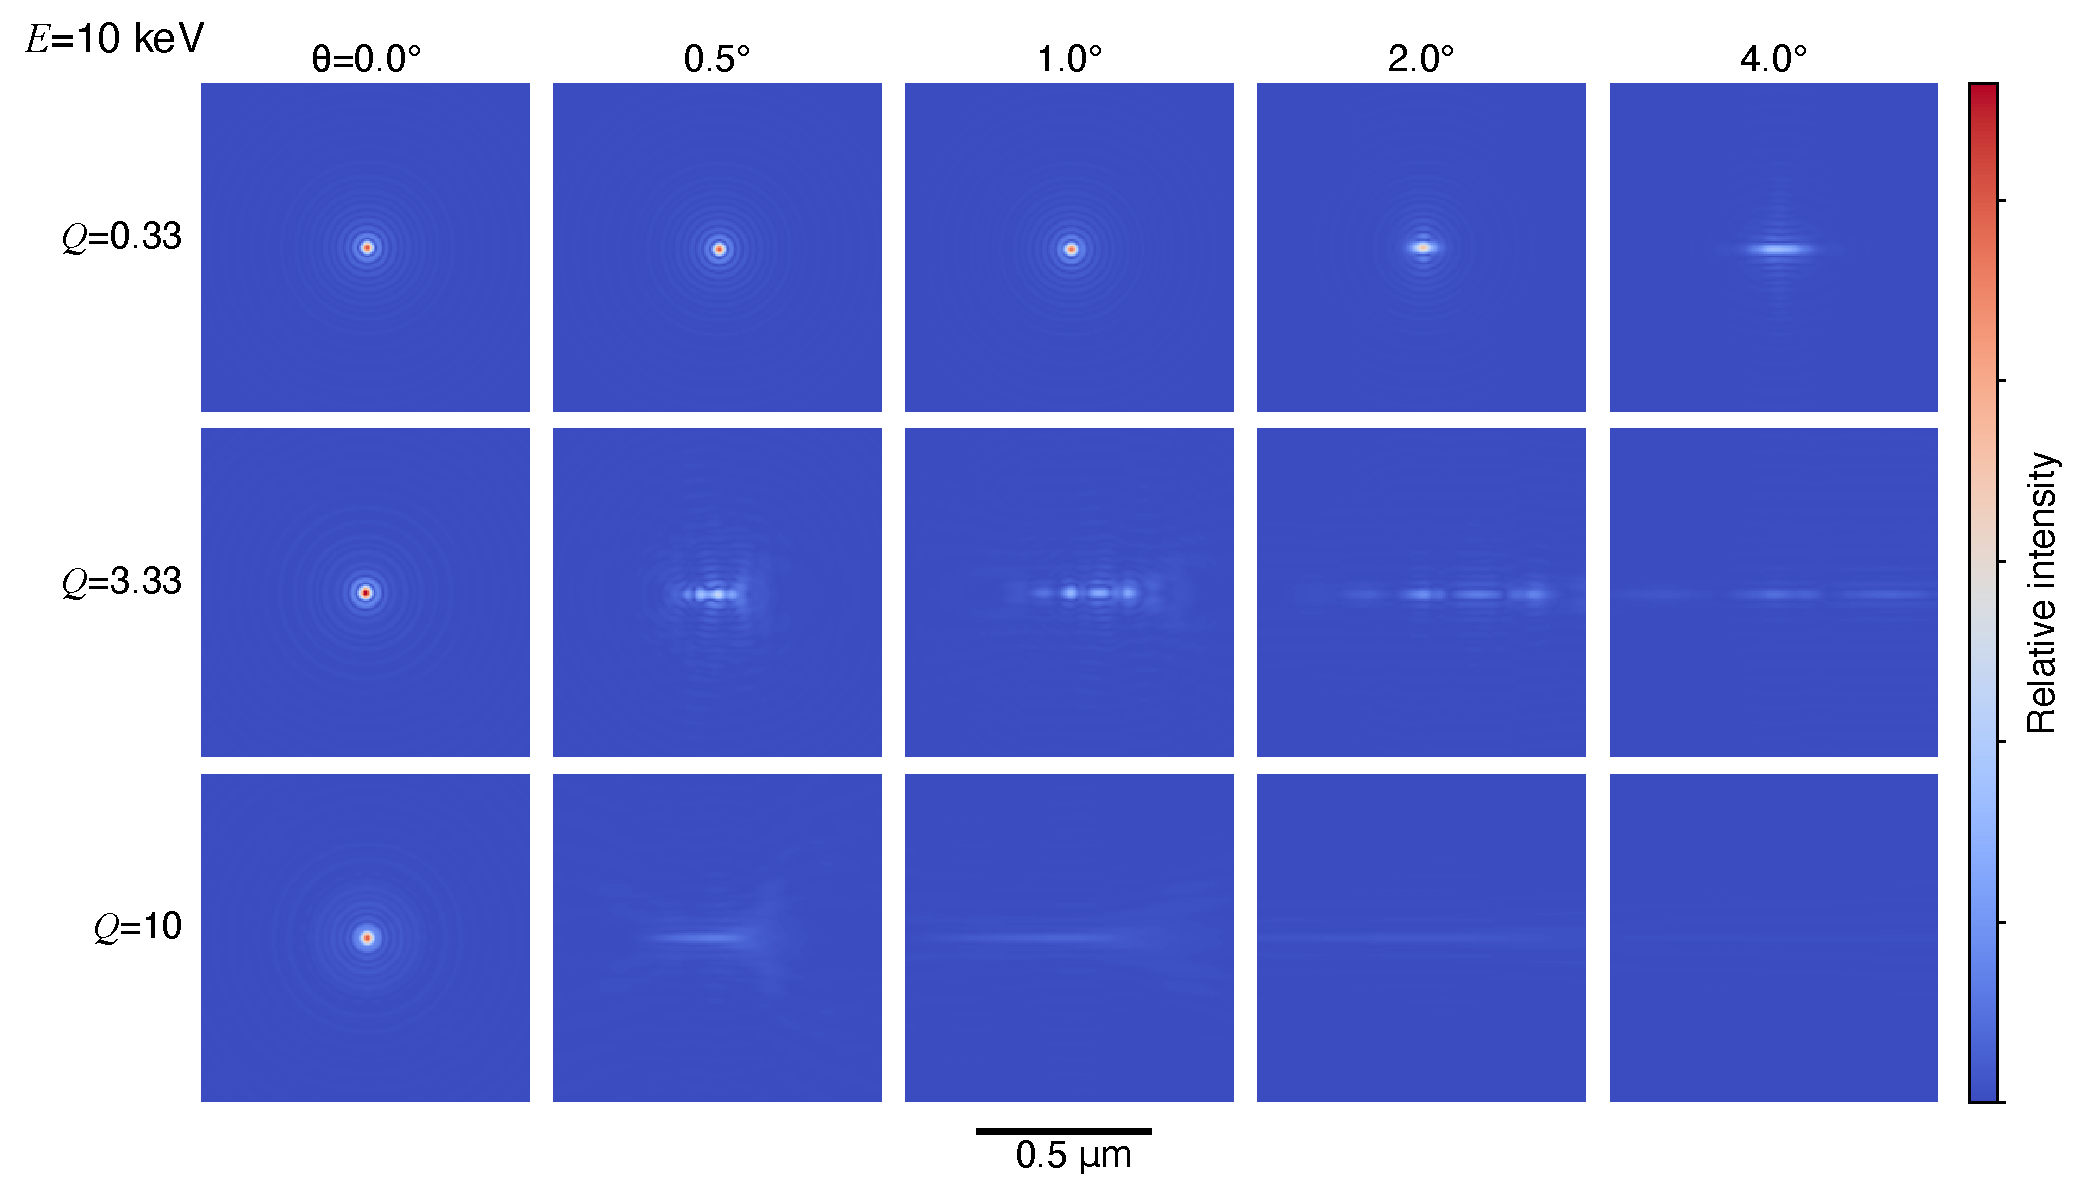
\includegraphics[scale=0.29]{foc_spot_ten}
				\caption{Focal Profile}	
			\end{figure}
		\end{center}

\end{frame}


\begin{frame}{Quantitative performance}
		\begin{center}
			\begin{figure}
				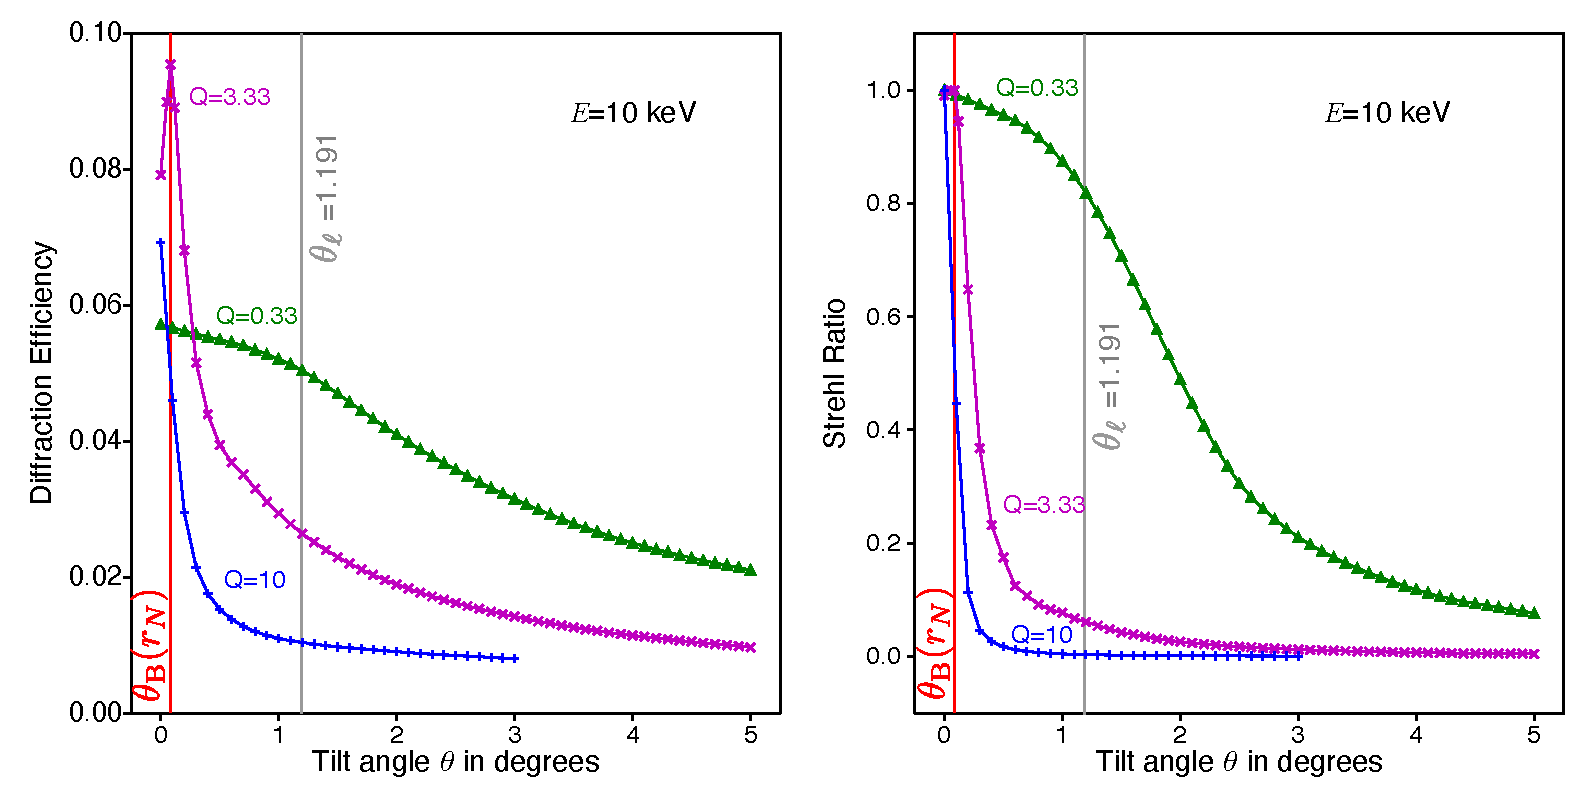
\includegraphics[scale=0.4]{tilt_plot_ten}
			\end{figure}
		\end{center}
\end{frame}


\begin{frame}{Summary}
	\begin{itemize}
		\item Systematic study of tilt misalignment conducted.
		\item Simple analytic models can predict misalignment limits and behavior for thin zone plates.
		\item Waveguide effects are important for thick zone plates.
	\end{itemize}
\end{frame}


\begin{frame}{Acknowledgements}
  \begin{itemize}
  \item \alert{Kenan Li} SLAC
  \item \alert{Michael Wojcik} APS,ANL.
  \item \alert{NIMH} U01 MH109100
  \end{itemize}
\end{frame}


%\end{comment}

% All of the following is optional and typically not needed. 
%\appendix
\renewcommand*{\bibfont}{\scriptsize}
\begin{frame}[t, allowframebreaks]
\frametitle{References}
\bibliographystyle{dinat-etal}
\bibliography{xsd_coffee_talk}
\end{frame}


\section{Backup}
\begin{frame}{Programming details}
	\begin{itemize}
		\item Implemented in Python3 using the scientific python stack : NumPy,SciPy
		\item FFT's via pyFFTW
		\item numexpr for pointwise multiplication
		\item libvips for 3D rotations
		\item HDF5 for I/O
	\end{itemize}

\end{frame}

\begin{frame}{Waveguide effects at no tilt}
	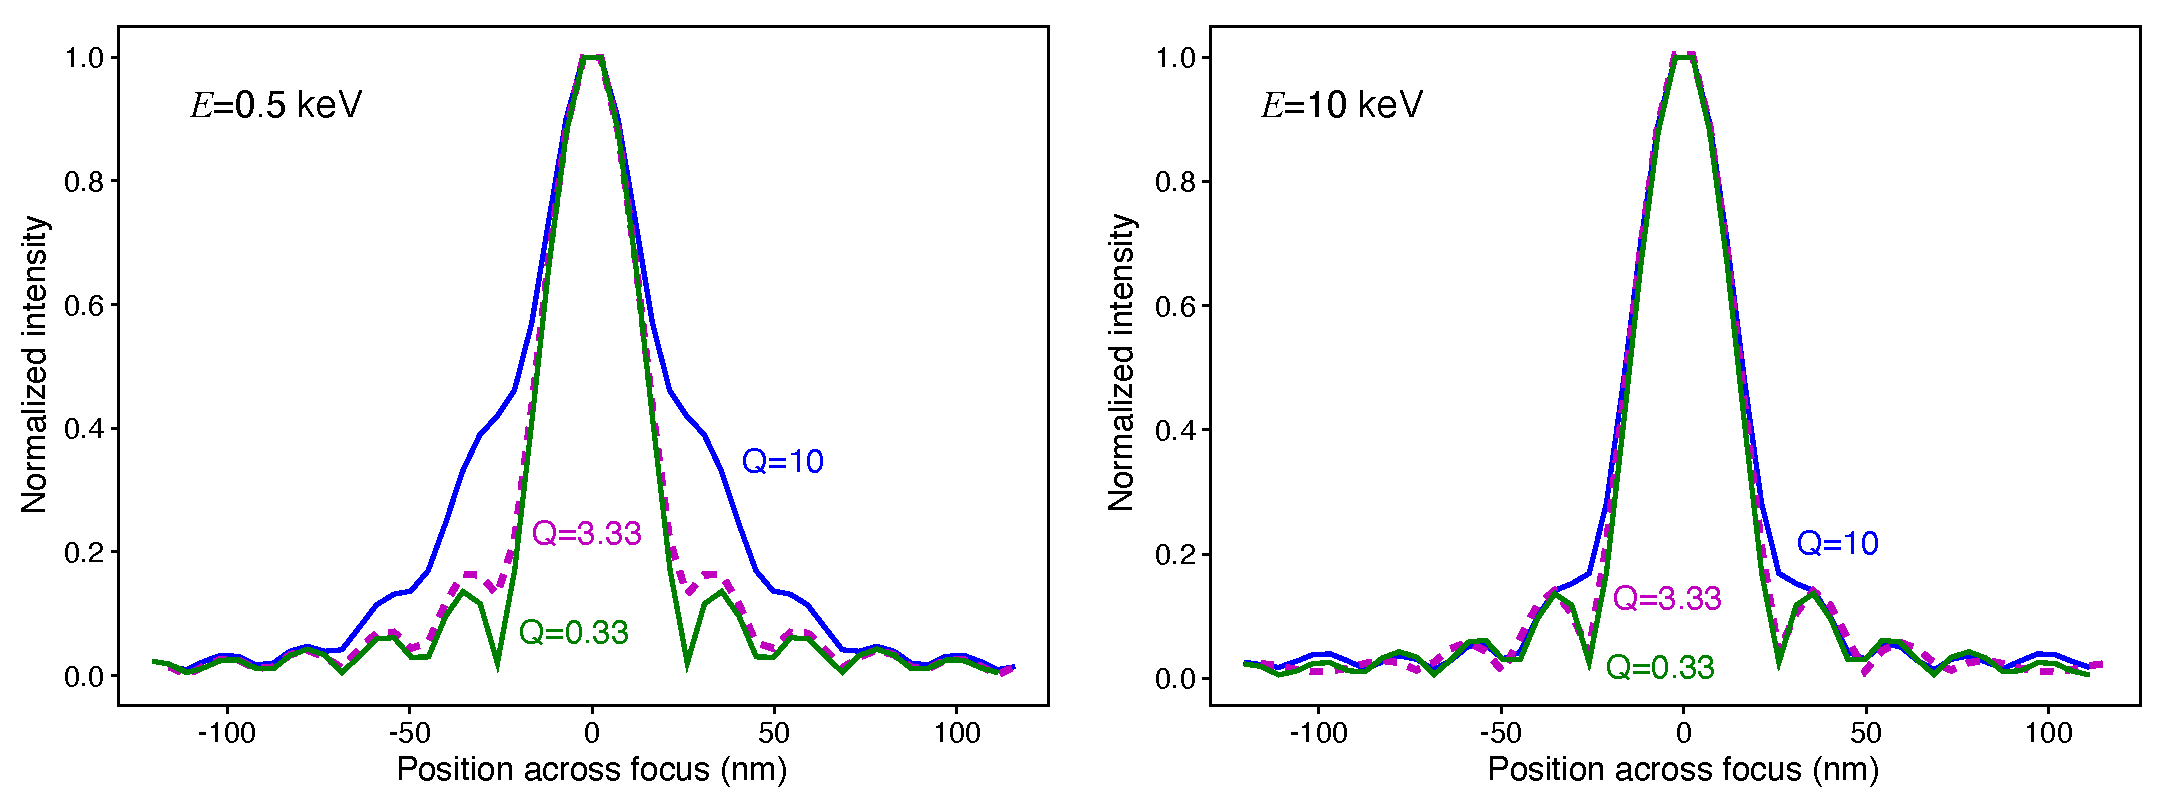
\includegraphics[scale=0.3]{foc_profiles}
\end{frame}

\end{document}

